    %% Beispiel-Präsentation mit LaTeX Beamer im KIT-Design
    %% entsprechend den Gestaltungsrichtlinien vom 1. August 2020
    %%
    %% Siehe https://sdqweb.ipd.kit.edu/wiki/Dokumentvorlagen
    
    %% Beispiel-Präsentation
    \documentclass{sdqbeamer} 
    \usepackage{booktabs}
    \usepackage{graphicx}
    \usepackage{xcolor}
    \usepackage{listings}
    \usepackage{tikz}
    \usepackage{amssymb}
    
    
    
    \lstdefinelanguage{GitLog}{
      morekeywords={feat,fix,chore,ci,Merge,draft},
      sensitive=false,
      morecomment=[l]{\#}
    }
    
    \lstset{
      language=GitLog,
      basicstyle=\ttfamily,
      keywordstyle=\color{blue},
      commentstyle=\color{gray},
      breaklines=true,
      columns=fullflexible,
      frame=single,
      keepspaces=true,
    }
    
    \AtBeginSection[]{
      \begin{frame}
      \vfill
      \centering
      \begin{beamercolorbox}[]{title}
        \centering\usebeamerfont{title}\huge\underline\insertsectionhead\par%
      \end{beamercolorbox}
      \vfill
      \end{frame}
    }
    
     
    %% Titelbild
    \titleimage{banner_2020_kit}
    
    %% Gruppenlogo
    %\grouplogo{mylogo} 
    
    %% Gruppenname und Breite (Standard: 50 mm)
    \groupname{Human-Computer Interaction and Accessibility}
    \groupnamewidth{50mm}
    \grouplogo{grouplogo.jpg}
    
    % Beginn der Präsentation
    
    \title[Solidarische Raumnutzung Implementierung]{Kolloquium Implementierung zur Solidarischen Raumnutzung}
    \subtitle{PSE-Projekt WS24/25} 
    \author[]{Alexander Klee, Jannik Hönlinger, Johannes Frohnmeyer, Ben Steinle und Antonia Ammon}
    
    \date{\today}
    
    % Literatur 
     
    \usepackage[citestyle=authoryear,bibstyle=numeric,hyperref,backend=biber]{biblatex}
    \addbibresource{presentation.bib}
    \bibhang1em
    
    \begin{document}
     
    %Titelseite
    \KITtitleframe
    
    %Inhaltsverzeichnis
    \begin{frame}{Inhaltsverzeichnis}
    \tableofcontents
    \end{frame}
    
    \section{Zeitplan}
    
    \subsection{GANTT Chart}
    \begin{frame}{\insertsubsectionhead}
        \begin{figure}
            \centering
            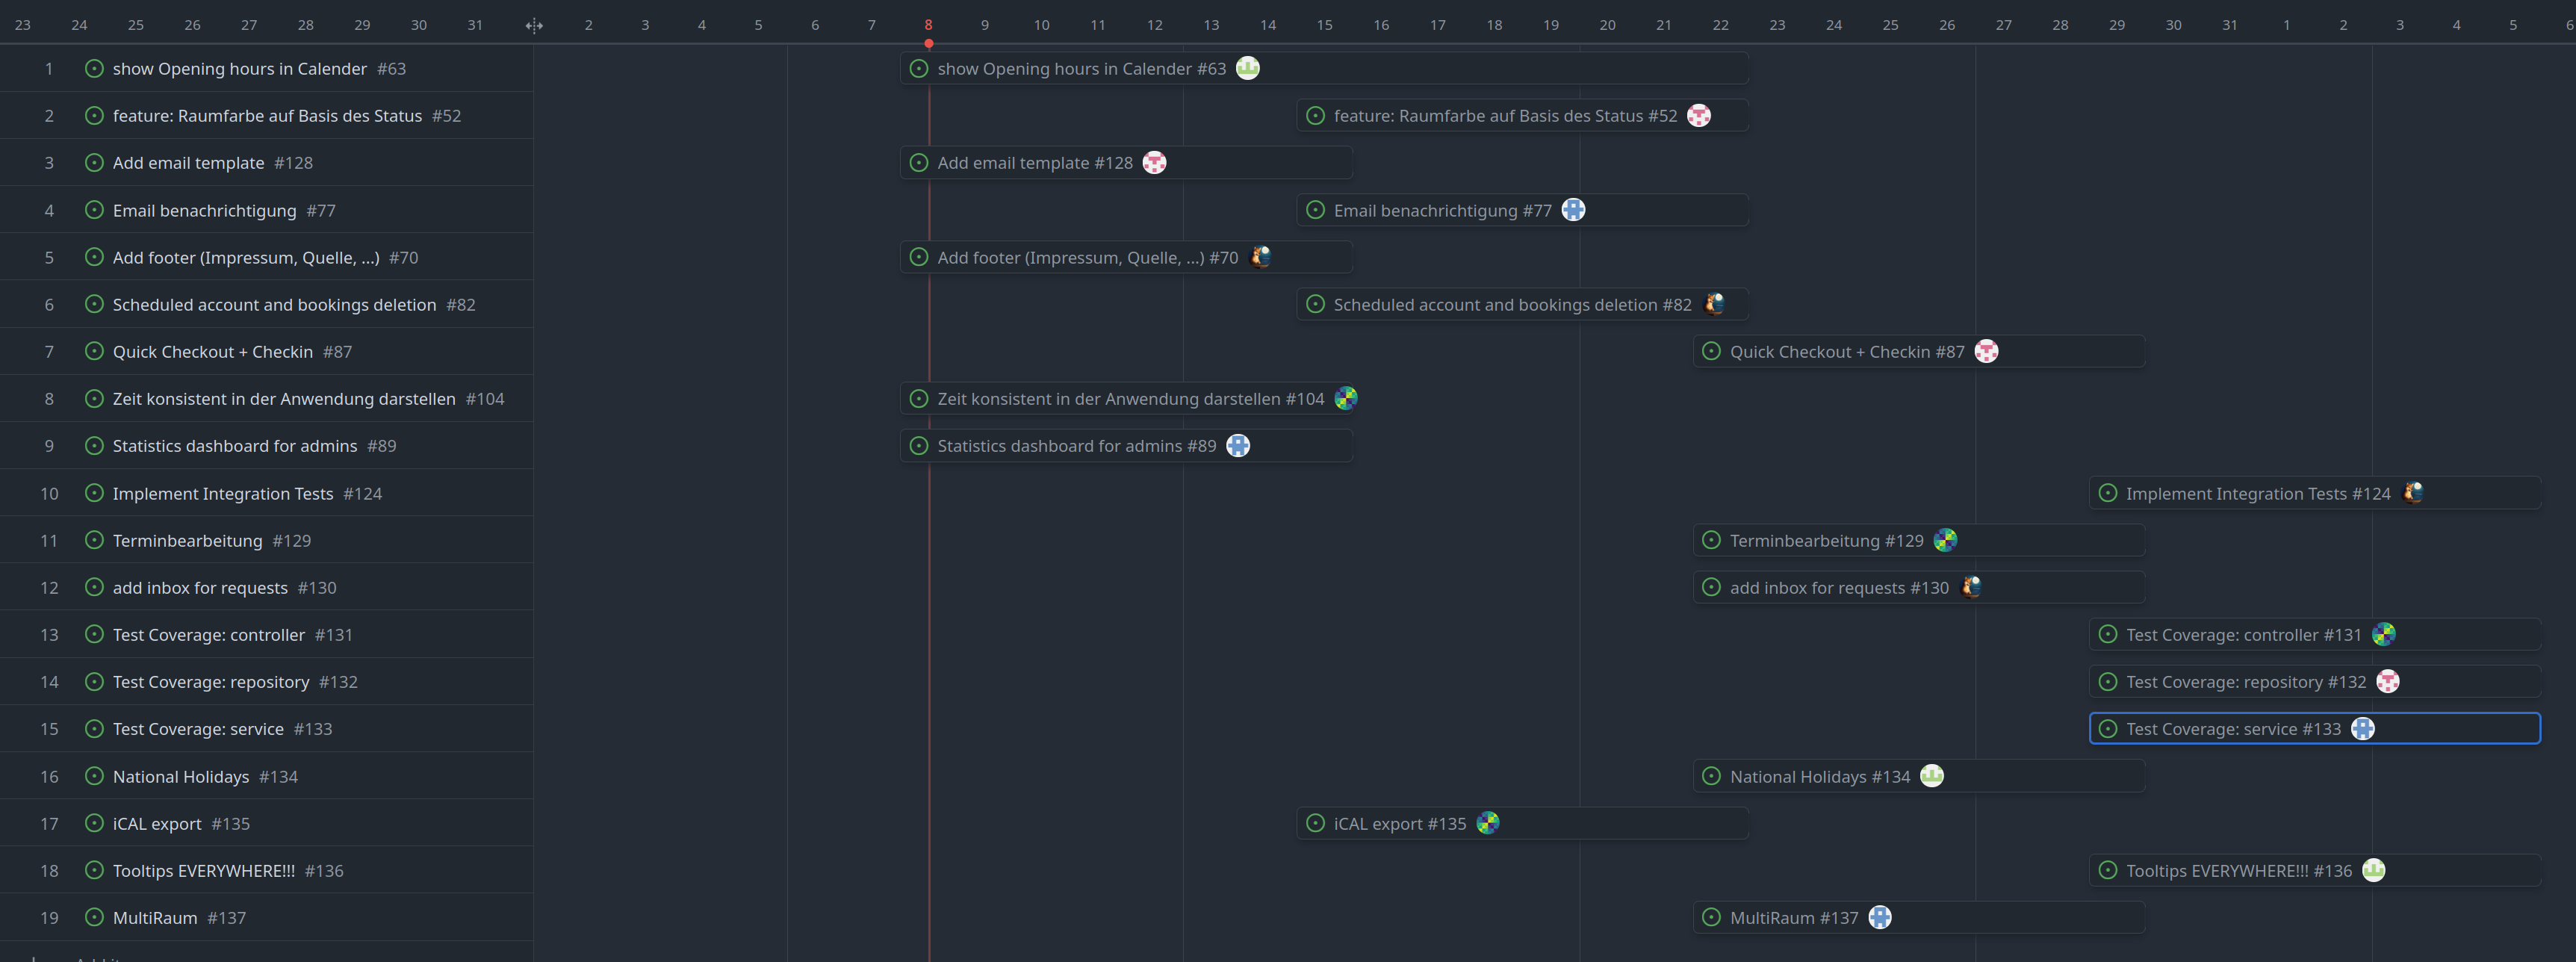
\includegraphics[width=1\linewidth]{tasks.png}
            \label{fig:enter-label}
        \end{figure}
    \end{frame}
    \subsection{Einhaltung des Zeitplans}
    \begin{frame}{Einhaltung des Zeitplans}
        \begin{itemize}
            \item Zeitplan wurde weitesgehend eingehalten
            \item Es kam vereinzelt zu Verzögerungen, war jedoch unkritisch
        \end{itemize}
    \end{frame}
    
    
    \section{Was wurde implementiert? (Auszug)}
    \begin{frame}{Kalendaransicht (Landing Page)}
        \thispagestyle{plain}
        \begin{figure}
            \centering
            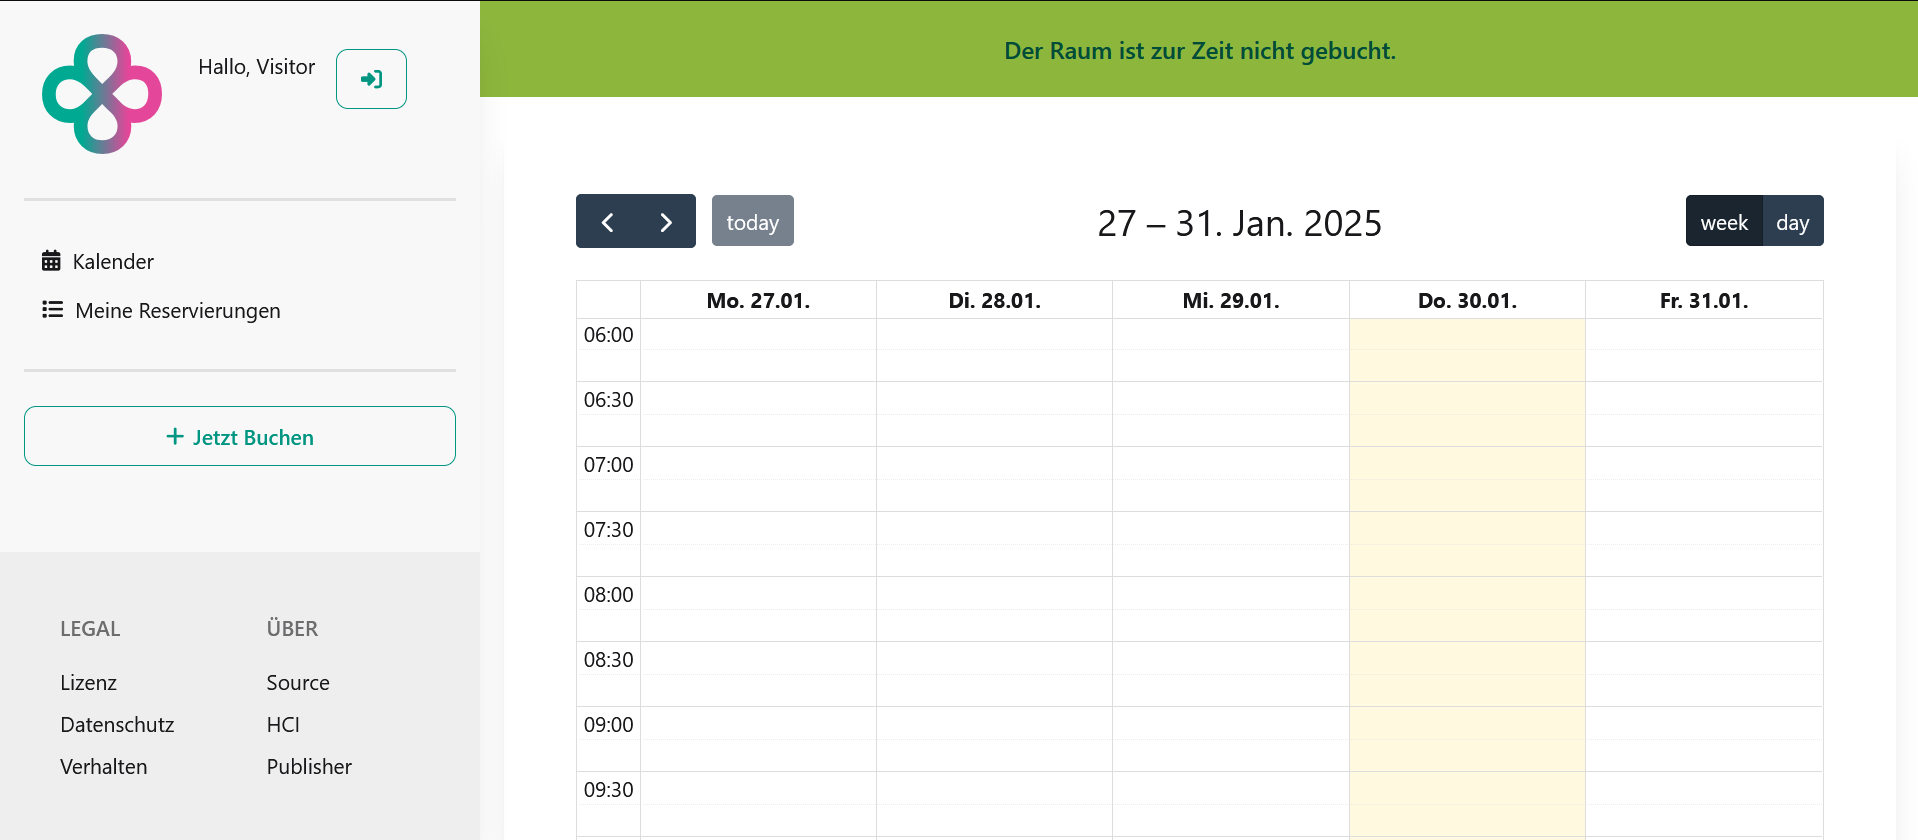
\includegraphics[width=1\linewidth]{calendar.png}
            \label{fig:enter-label}
        \end{figure}
        
    \end{frame}
    
    \begin{frame}{Kalenderansicht im Darkmode}
        \thispagestyle{plain}
        \begin{figure}
            \centering
            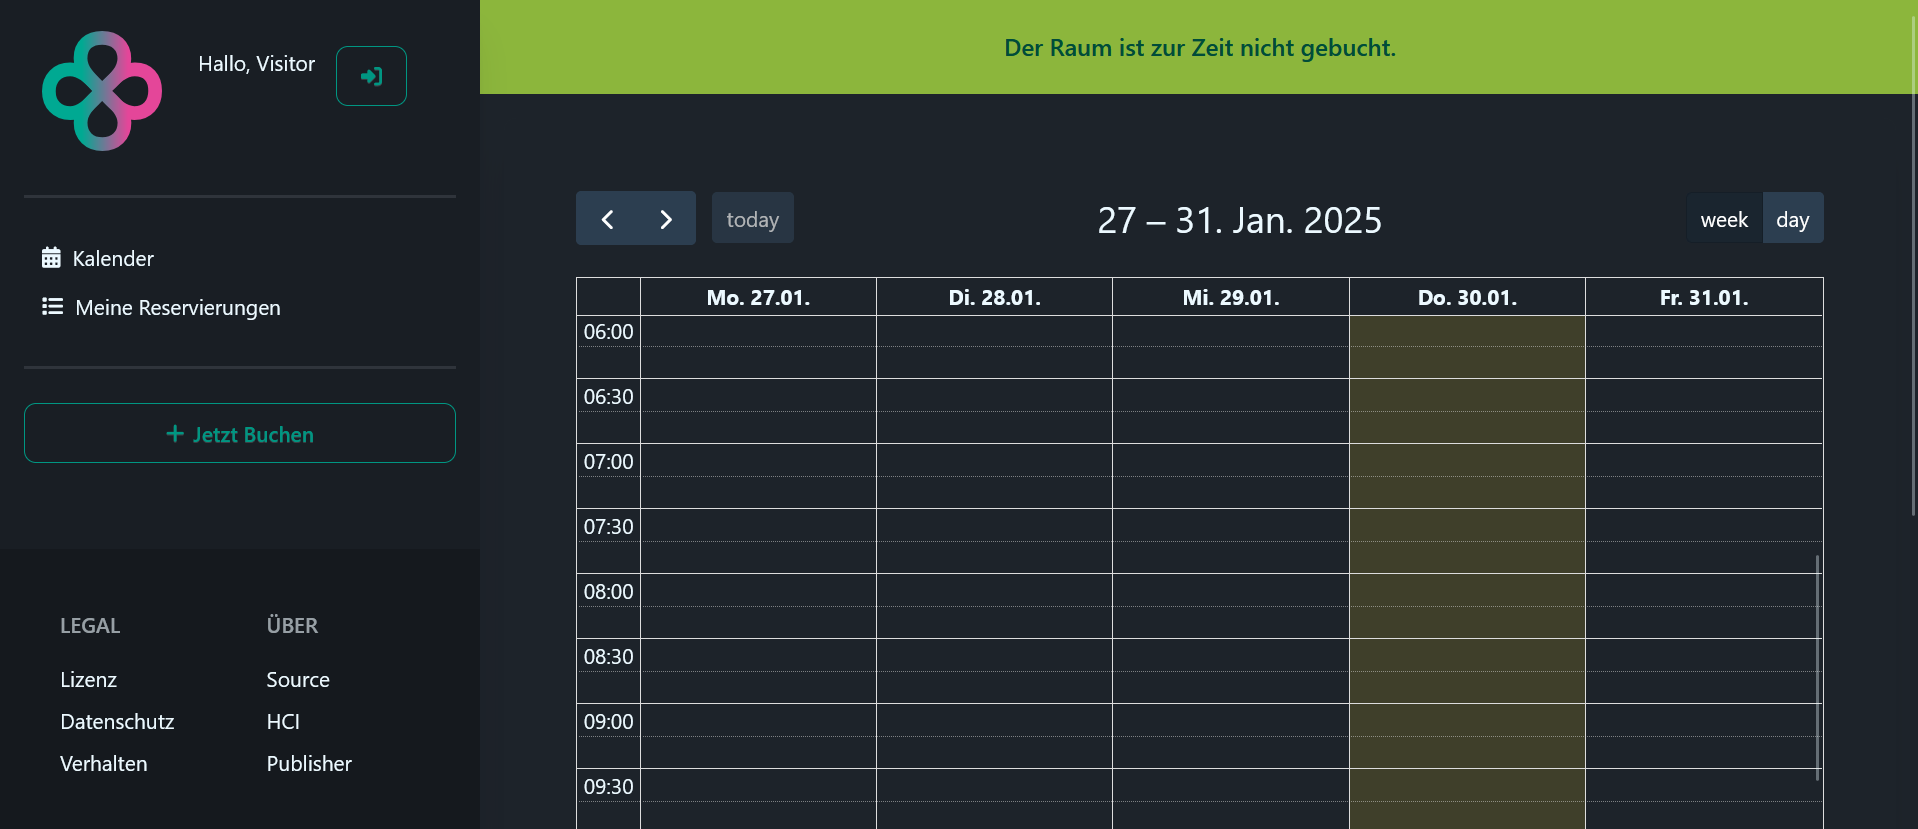
\includegraphics[width=1\linewidth]{calendar_dark.png}
            \label{fig:enter-label}
        \end{figure}
    \end{frame}
    
    \begin{frame}{Termin erstellen}
        \thispagestyle{plain}
        \begin{figure}
            \centering
            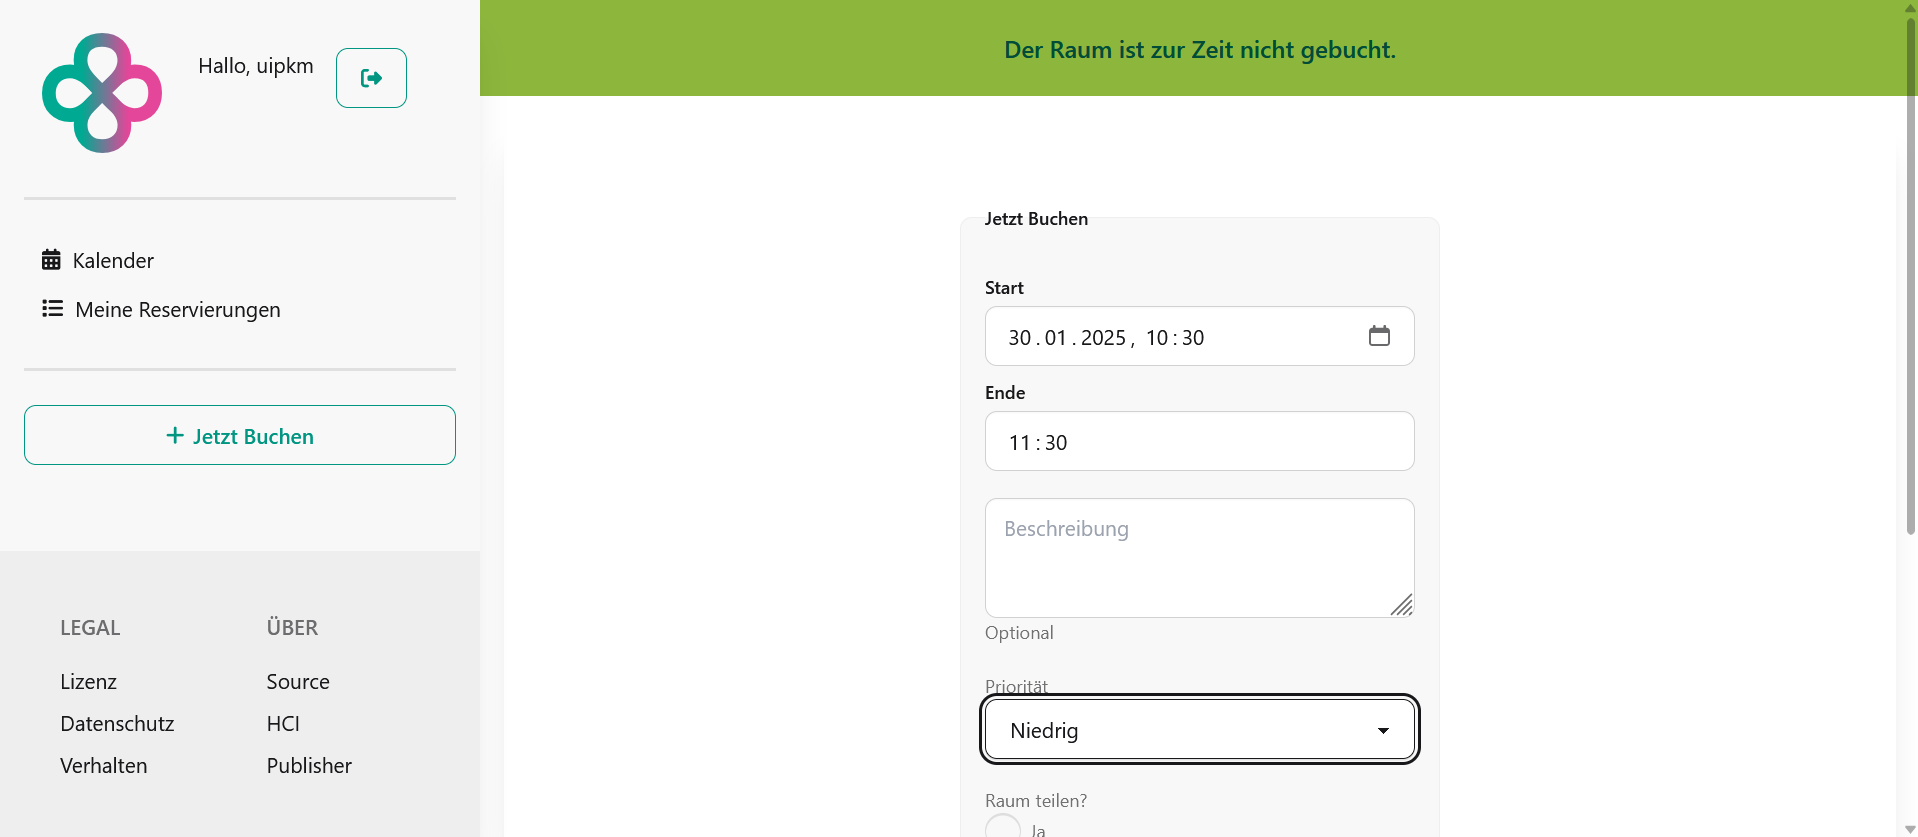
\includegraphics[width=1\linewidth]{bookings_create_form_1.png}
            \label{fig:enter-label}
        \end{figure}
    \end{frame}
    
    \begin{frame}{Termin erstellen}
        \thispagestyle{plain}
        \begin{figure}
            \centering
            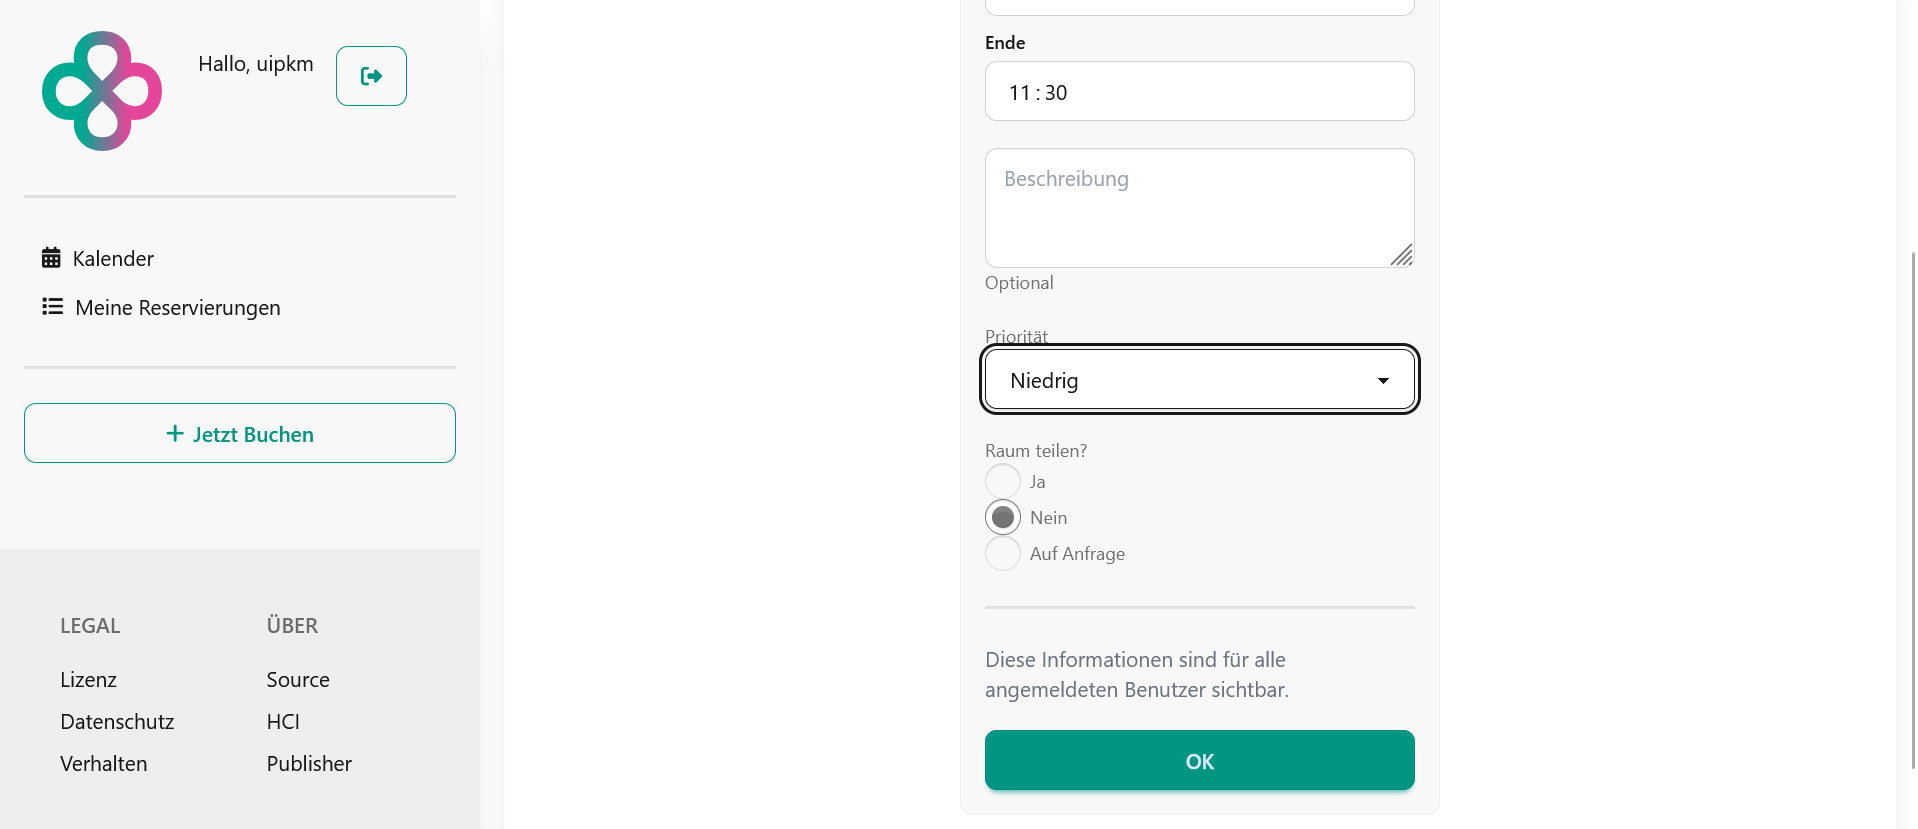
\includegraphics[width=1\linewidth]{bookings_create_form_2.png}
            \label{fig:enter-label}
        \end{figure}
    \end{frame}
    
    \begin{frame}{Anmeldeseite}
        \thispagestyle{plain}
        \begin{figure}
            \centering
            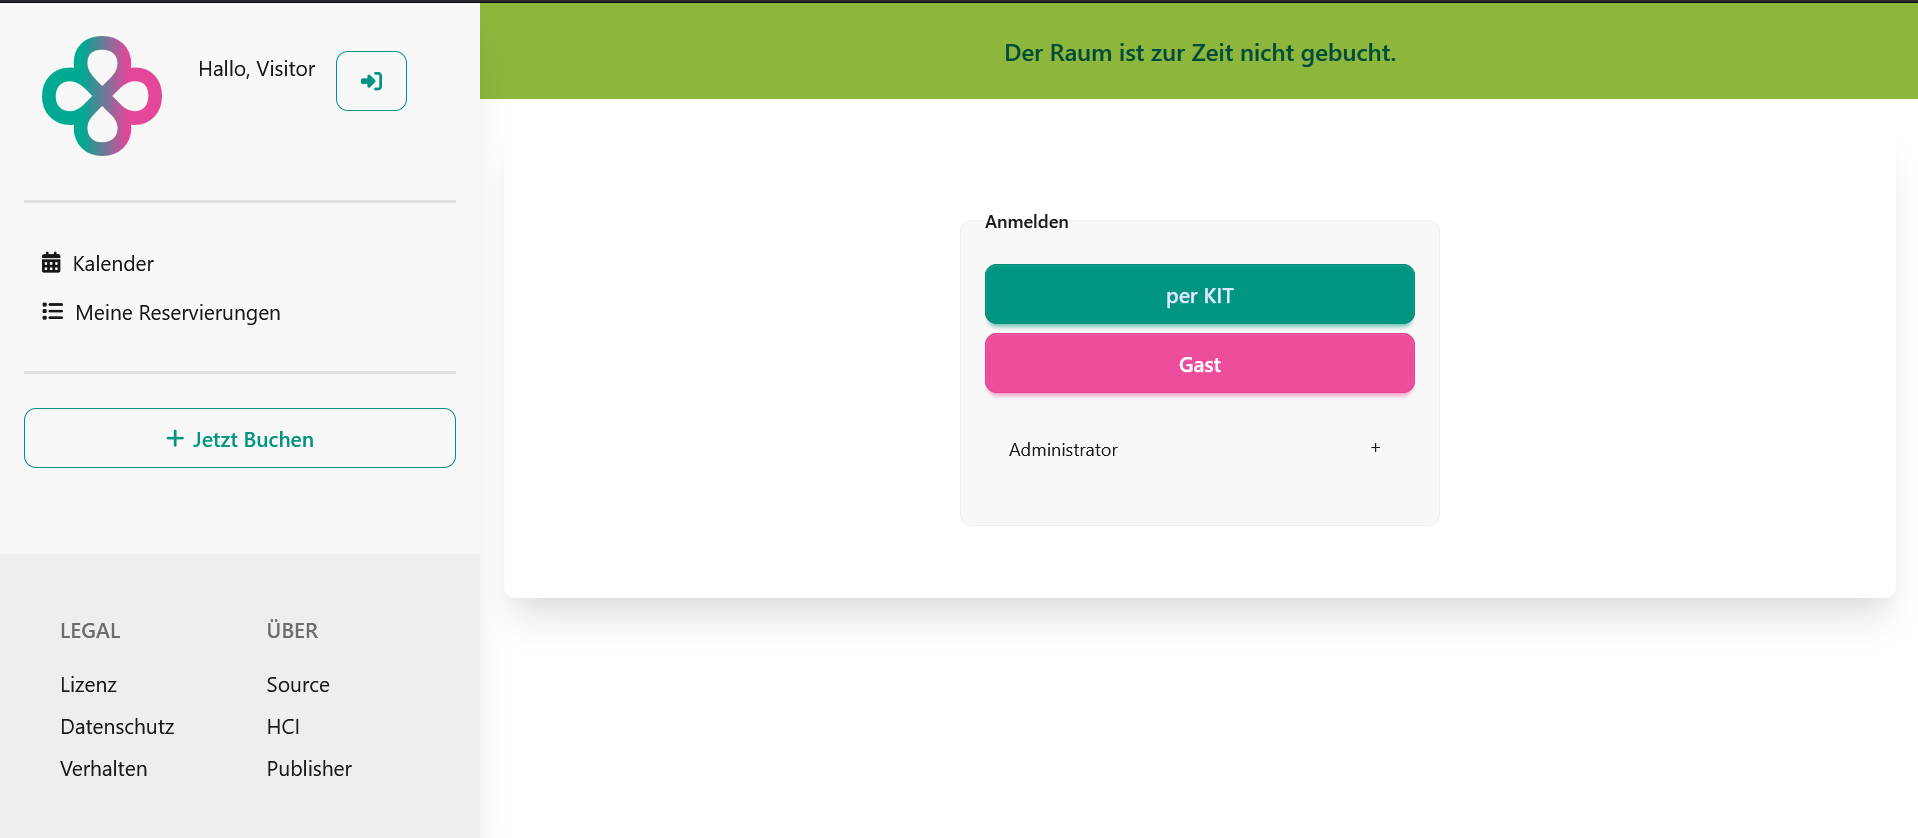
\includegraphics[width=1\linewidth]{auth_login.png}
            \caption{Login}
            \label{fig:enter-label}
        \end{figure}
    \end{frame}
    
    \begin{frame}{Reservierungsübersicht}
        \thispagestyle{plain}
        \begin{figure}
            \centering
            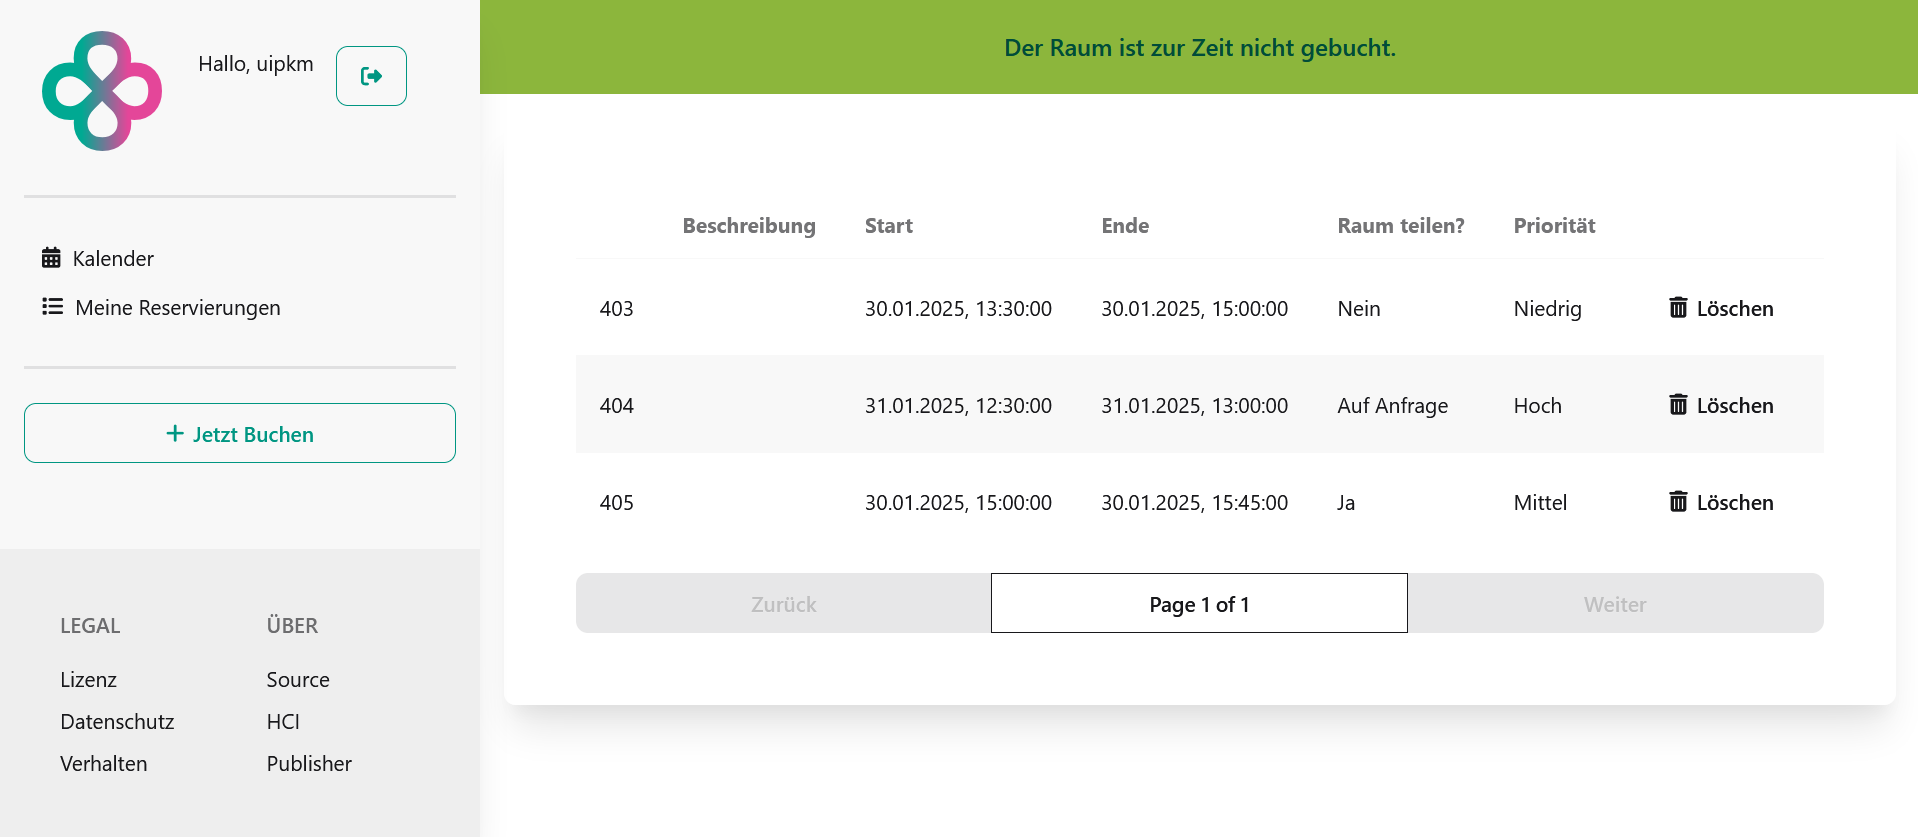
\includegraphics[width=1\linewidth]{bookings_list.png}
            \label{fig:enter-label}
        \end{figure}
    \end{frame}
    
    \begin{frame}{Reservierung im Kalender}
        \thispagestyle{plain}
        \begin{figure}
            \centering
            
\includegraphics[width=1\linewidth]{bookings_single.png}
            \label{fig:enter-label}
        \end{figure}
    \end{frame}
    
    \begin{frame}{Quick Checkout Button}
        \thispagestyle{plain}
        \begin{figure}
            \centering
            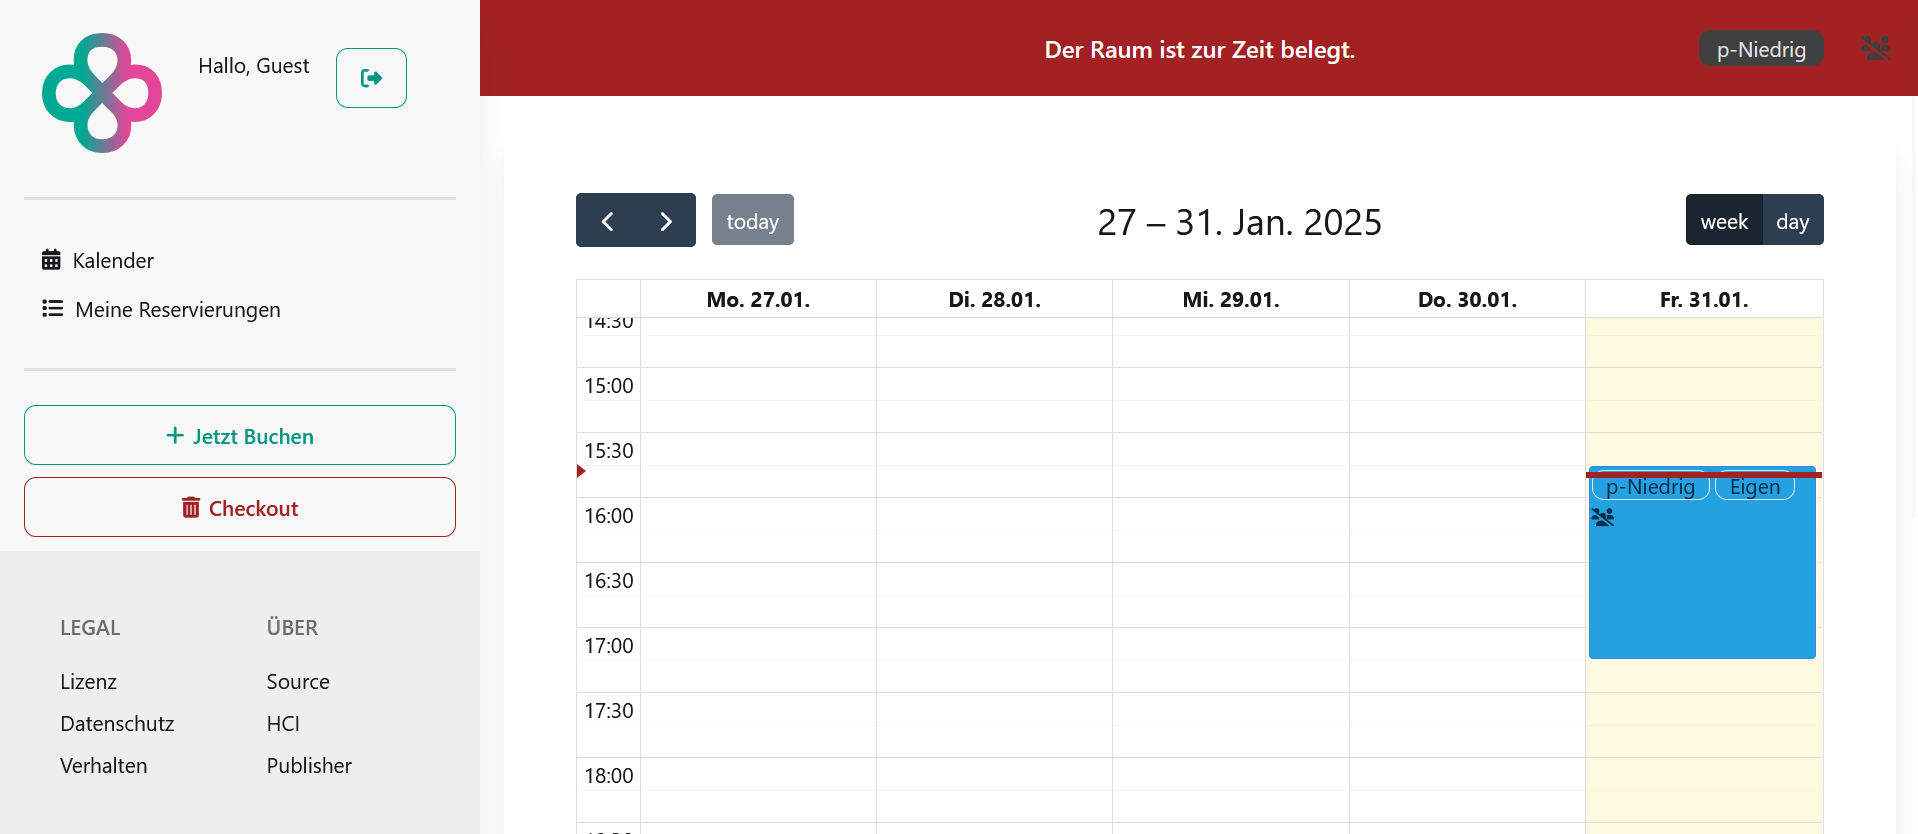
\includegraphics[width=1\linewidth]{check_out_button_light.png}
            \label{fig:enter-label}
        \end{figure}
    \end{frame}
    
    \begin{frame}{Kontenliste}
        \thispagestyle{plain}
        \begin{figure}
            \centering
            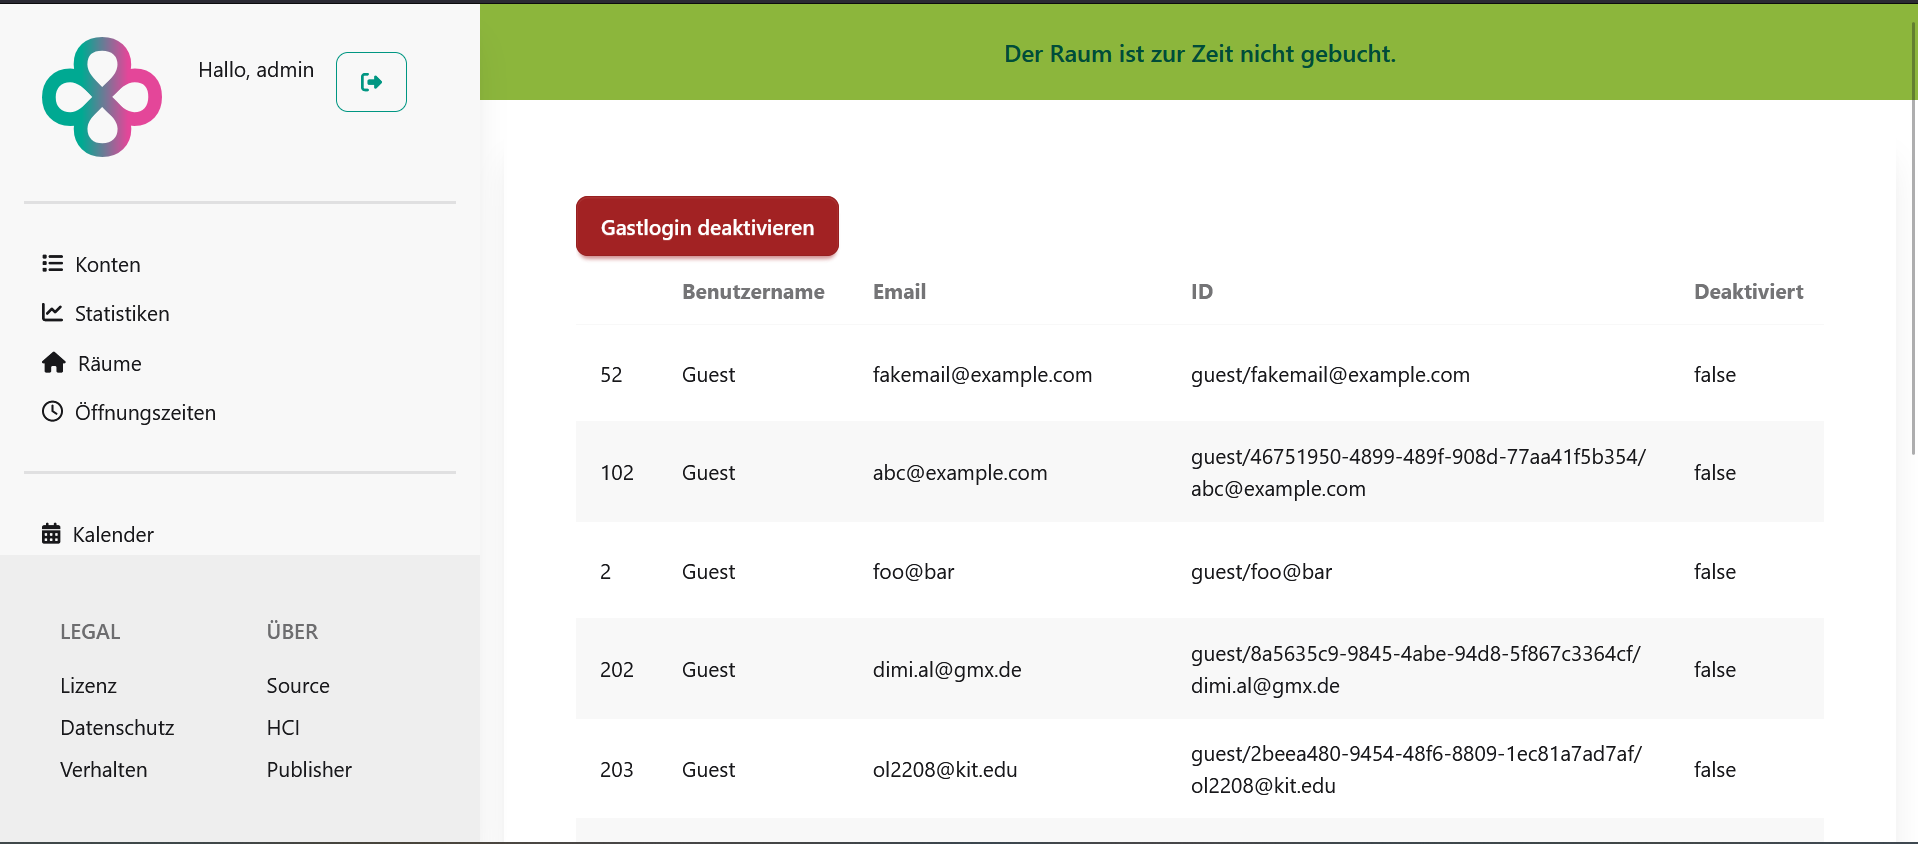
\includegraphics[width=1\linewidth]{admin_users.png}
            \label{fig:enter-label}
        \end{figure}
        
    \end{frame}
    
    \begin{frame}{Statistikansicht}
        \thispagestyle{plain}
        \begin{figure}
            \centering
            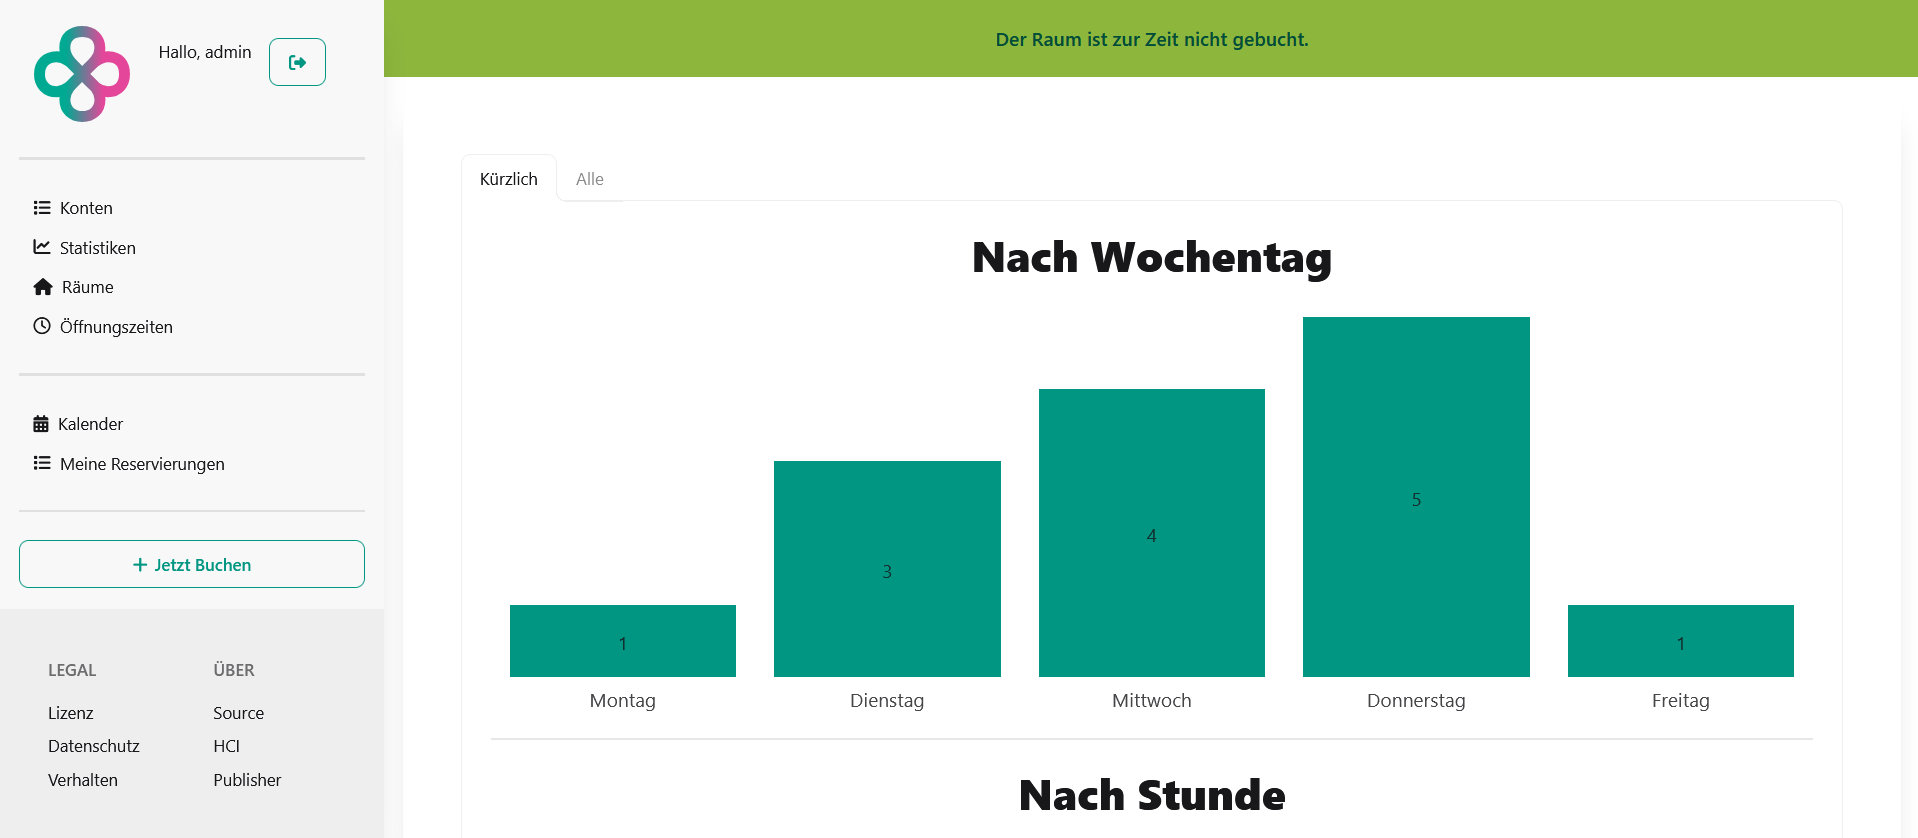
\includegraphics[width=1\linewidth]{admin_statistics.png}
            \label{fig:enter-label}
        \end{figure}
    \end{frame}
    
    \begin{frame}{Konfiguration von Öffungszeiten}
        \thispagestyle{plain}
        \begin{figure}
            \centering
            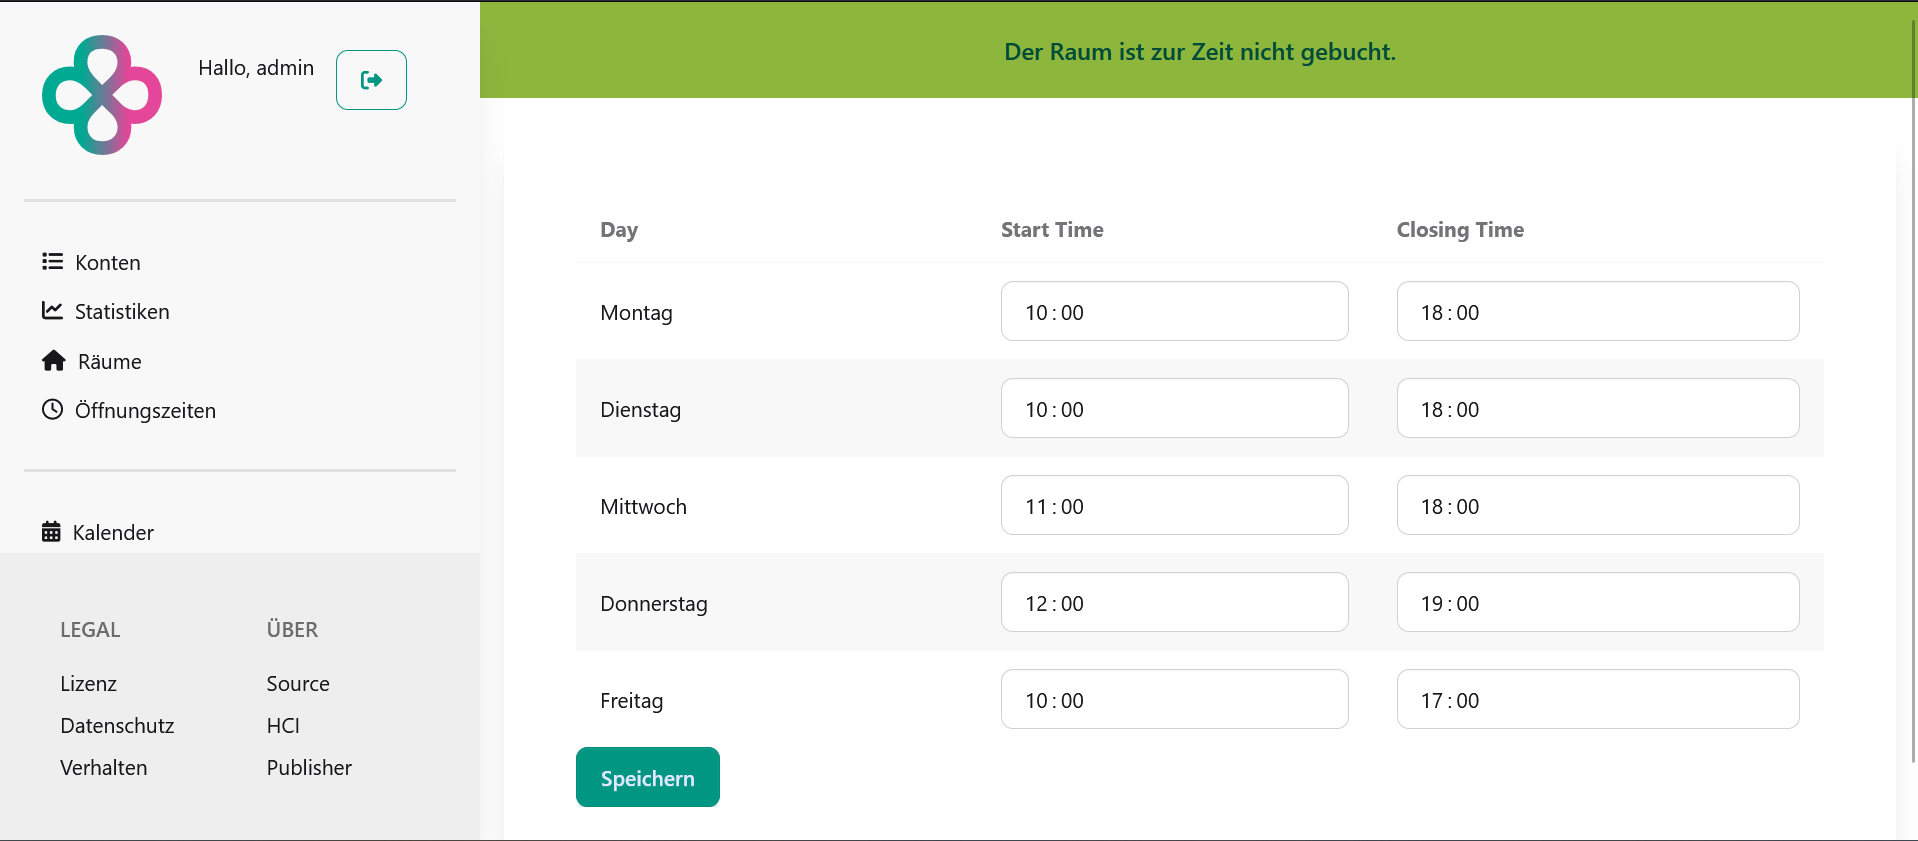
\includegraphics[width=1\linewidth]{admin_opening_hours.png}
            \label{fig:enter-label}
        \end{figure}
    \end{frame}
    
    \begin{frame}{Öffungszeiten im Kalender}
        \thispagestyle{plain}
        \begin{figure}
            \centering
            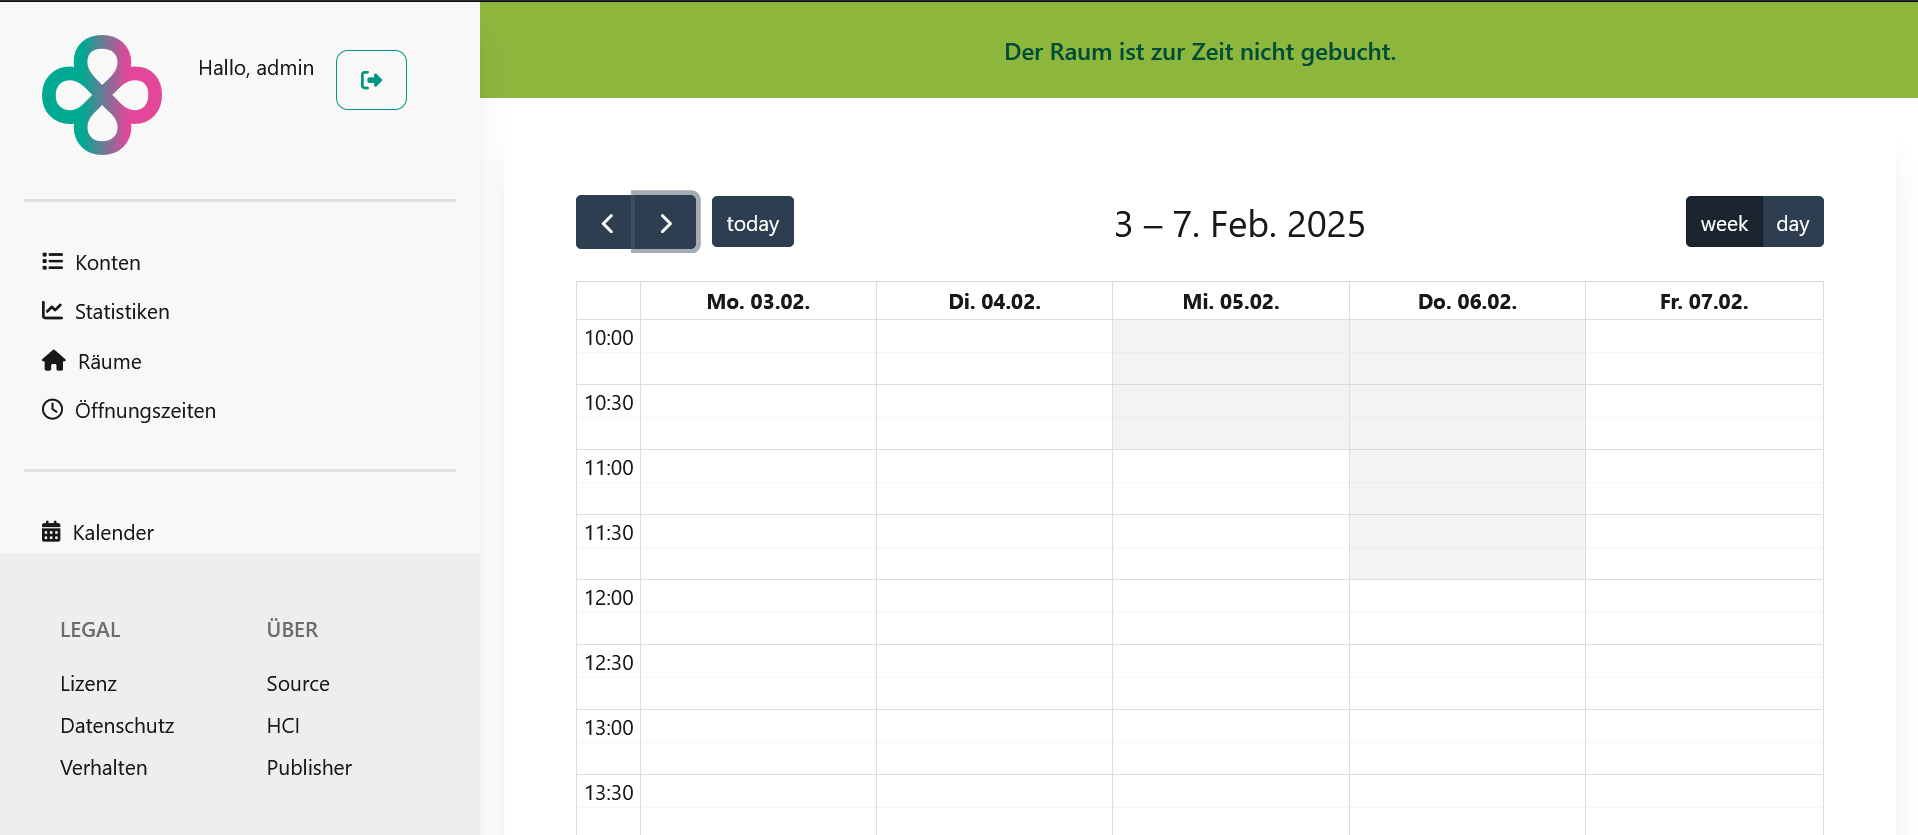
\includegraphics[width=1\linewidth]{calendar_opening_hours.png}
            \label{fig:enter-label}
        \end{figure}
    \end{frame}
    
    \subsection{Was wurde nicht implementiert?}
    \begin{frame}{Welche Wunschkritierien wurde nicht implementiert?}
    
        \begin{itemize}
           \item Admins könnten die Möglichkeit haben, geplante Wartungs- und Sperrzeiten einzurichten
           \item Es könnte einen physischen Panik-Button geben. 
           \item Die Anwendung könnte in der Lage sein, Nutzende zu informieren, falls ein gewünschter Termin frei wird.
        \end{itemize}
       
        
        \hfill \break
        \hfill \break
        $\implies$ Alle anderen Kriterien wurde implementiert.
    \end{frame}
    
    
    \section{Änderungen zum Entwurf}
    \begin{frame}{ER Diagramm}
        \thispagestyle{plain}
    \begin{columns}
        \column{.2\textwidth}
        \begin{figure}
           
            \centering
        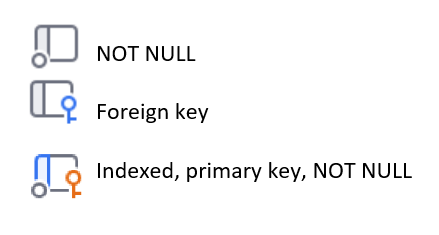
\includegraphics[width=1\linewidth]{ERLegend.png}
    \caption{Legende ER-Diagramm}
        \label{fig:enter-label}
        \end{figure}
        \column{.8\textwidth}
         \begin{figure}
            \centering
            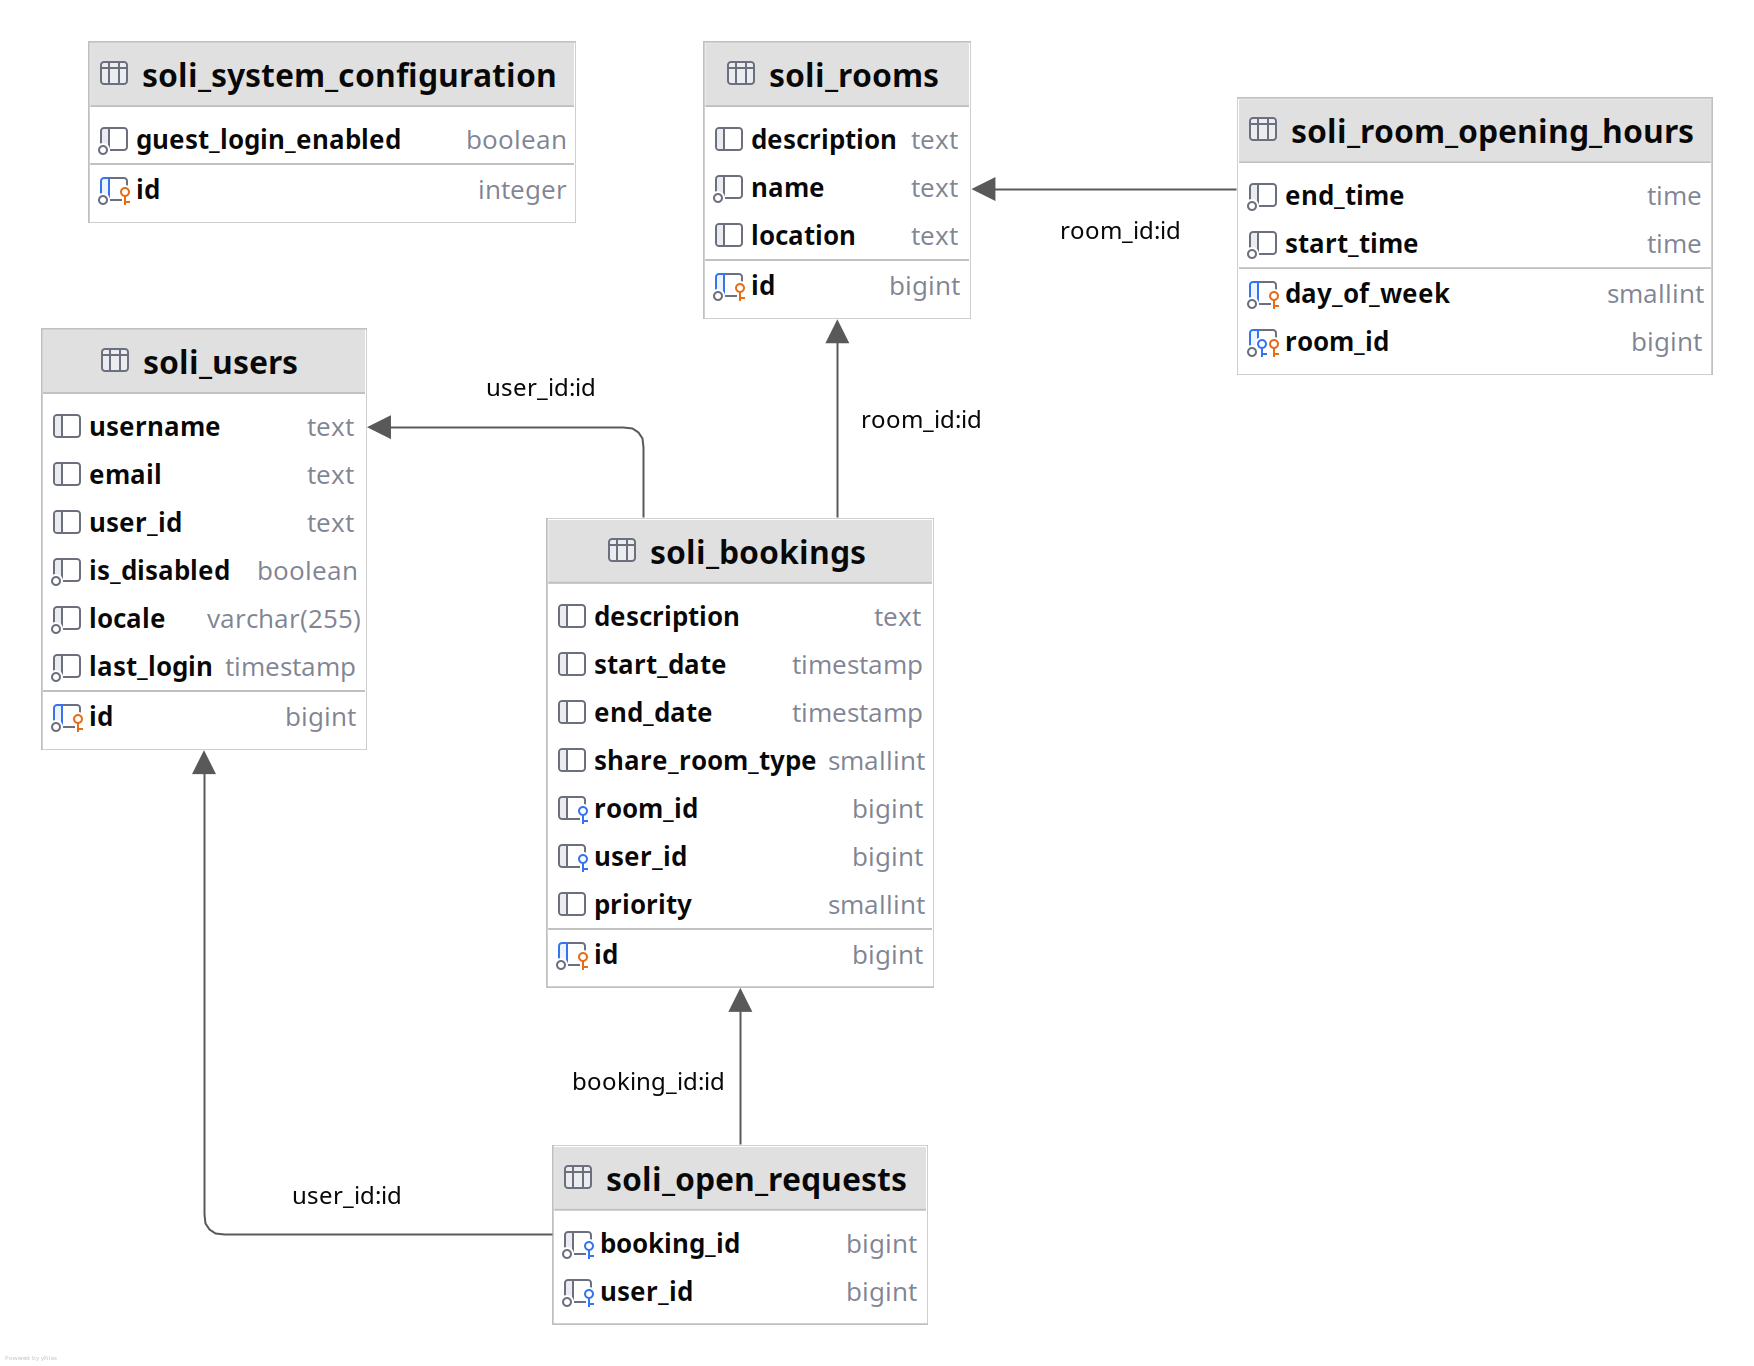
\includegraphics[width=0.75\linewidth]{database_new.png}
            \label{fig:enter-label}
        \end{figure}
    \end{columns}
    
    
       
    \end{frame}
    
    \begin{frame}{Klassendiagramm}
        Beim Klassendiagram wurde auch nachgebessert
        \hfill \break
        \hfill \break
        $\implies$ \url{https://solidarische-raumnutzung.github.io/solidarische-raumnutzung/classes.png} 
    \end{frame}
    
    \section{Statistiken des Projekts}
    
    \begin{frame}{Lines of Code / Commits}
        \thispagestyle{plain}
        \begin{columns}
            \column{.3\textwidth}
             \begin{table}[h]
        \centering
        \begin{tabular}{lr}
            \toprule
            Language & Code \\
            \midrule
            Java        & 5535 \\
            JTE        & 1213 \\
            CSS         & 236  \\
            Properties  & 235  \\
            SQL        & 141  \\
            SVG        & 92   \\
            YAML       & 70   \\
            JSON       & 14   \\
            Text       & 4    \\
            \midrule
            \textbf{Summe:} & 7540 \\
            \bottomrule
        \end{tabular}
        \caption{Statistik der Quellcodedateien}
        \label{tab:code_stats}
    \end{table}
        \column{.3\textwidth}
        \begin{figure}
            \centering
            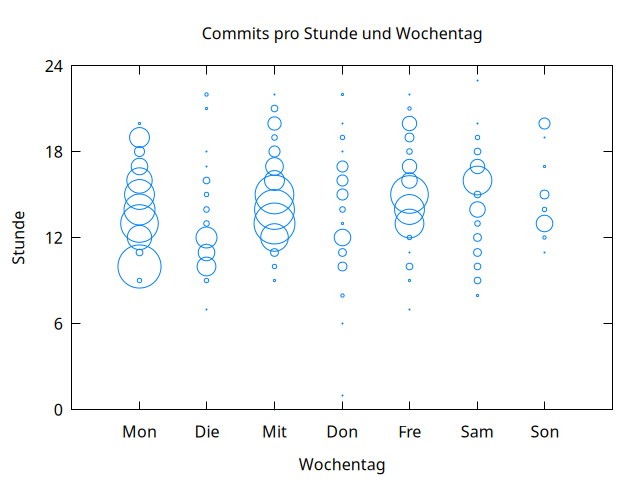
\includegraphics[width=1\linewidth]{hours.png}
            \caption{Commits pro Stunde und Wochentag}
            \label{fig:enter-label}
        \end{figure}
        In Summe $951$ Commits
        \hfill \break
        \hfill \break
        \hfill \break
        \hfill \break
        \end{columns}
      
    \end{frame}
    
    \begin{frame}{Commits over time}
        \begin{figure}
            \centering
            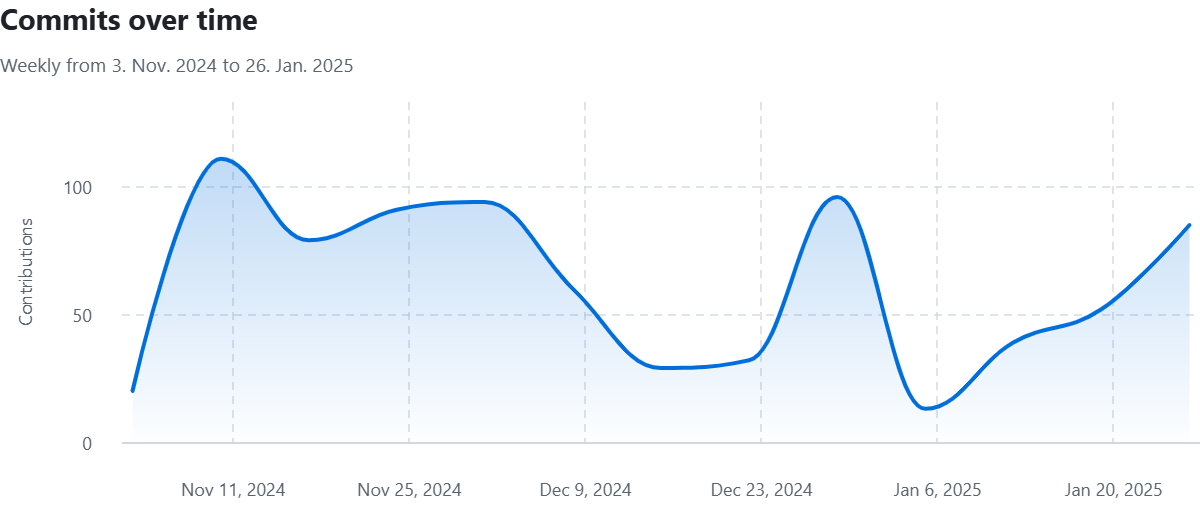
\includegraphics[width=0.8\linewidth]{Commits over time.png}
            \label{fig:enter-label}
        \end{figure}
    \end{frame}
    
    \section{Entwicklungsmodell}
    
    \begin{frame}{Entwicklungsmodell}
        \begin{columns}
            \column{.5\linewidth}
            \begin{itemize}
            \item Conventional Commits (fix, feat, ...)
            \item Arbeiten auf feature Branches $\implies$ Code-Reviews
            \item CI builds und automatisiertes Testen für jede Pull Request 
            \item Jede Änderung an Source Code wurde durch entsprechende Integration und Unit Tests gerechtfertigt $\implies$ Bereits jetzt schon Hohe Coverage (ca. 150 Unit- und Integrationtests)
            
        \end{itemize}
        \column{.5\linewidth}
            \begin{table}[h]
        \centering
        \renewcommand{\arraystretch}{1.3}
        \begin{tabular}{l|c}
            \textbf{Paket} & \textbf{Line Coverage} \\
            \hline
            \hline
            \textit{Controller}  & 69\% \\
            \textit{Domain}      & 87\% \\
            \textit{DTO}         & 79\% \\
            \textit{Filter}      & 100\% \\
            \textit{Repository}  & 100\% \\
            \textit{Service}     & 85\% \\
            \hline
            \textit{Gesamt}      & 76\% \\
        \end{tabular}
        \label{tab:progress}
    \end{table}
        \end{columns}
        
    \end{frame}
    
    
    \begin{frame}{Code Reviews / Pull Reqeusts}
        \thispagestyle{plain}
    \begin{figure}
        \centering
        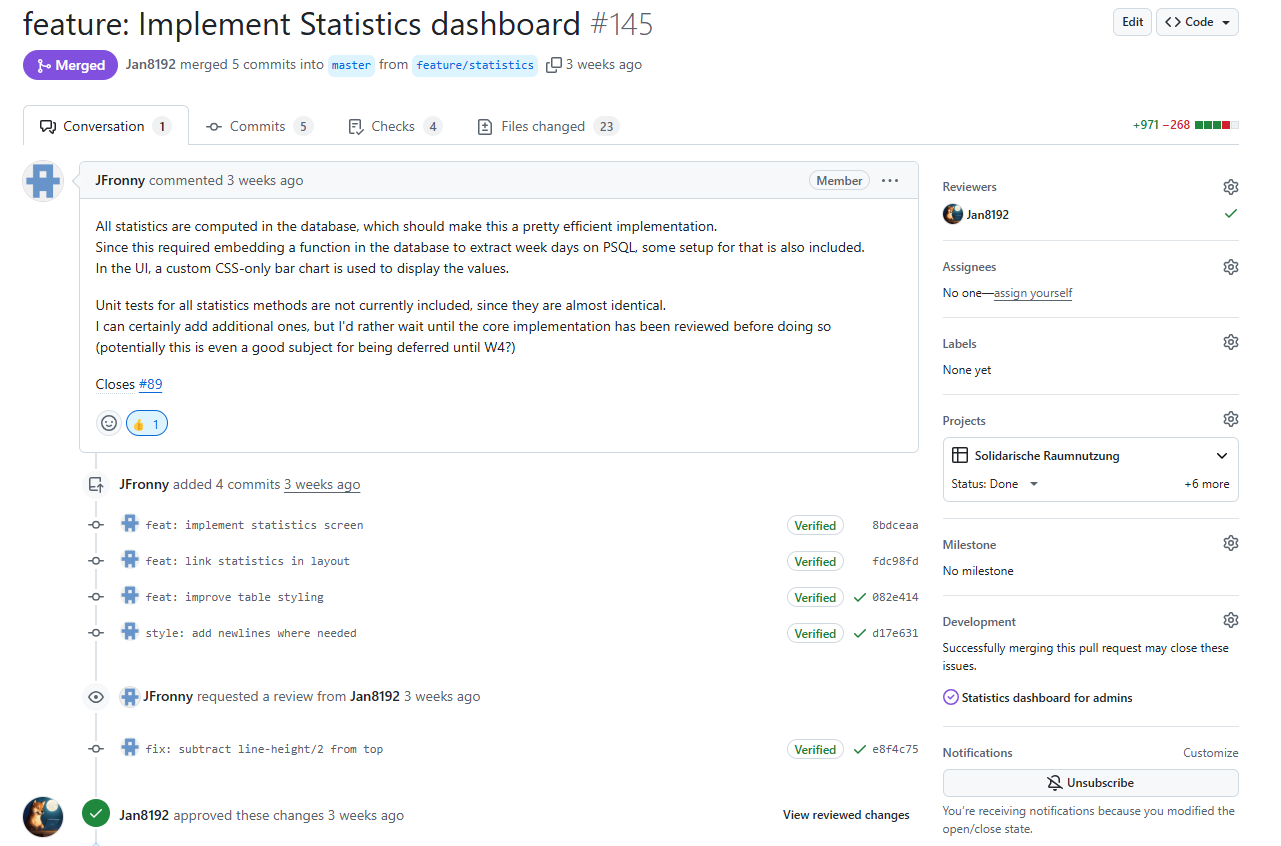
\includegraphics[width=1\linewidth]{pr_reviews.png}
        \label{fig:enter-label}
    \end{figure}
    \end{frame}
    
    \begin{frame}{Commit History}
        \thispagestyle{plain}
        \begin{figure}
            \centering
            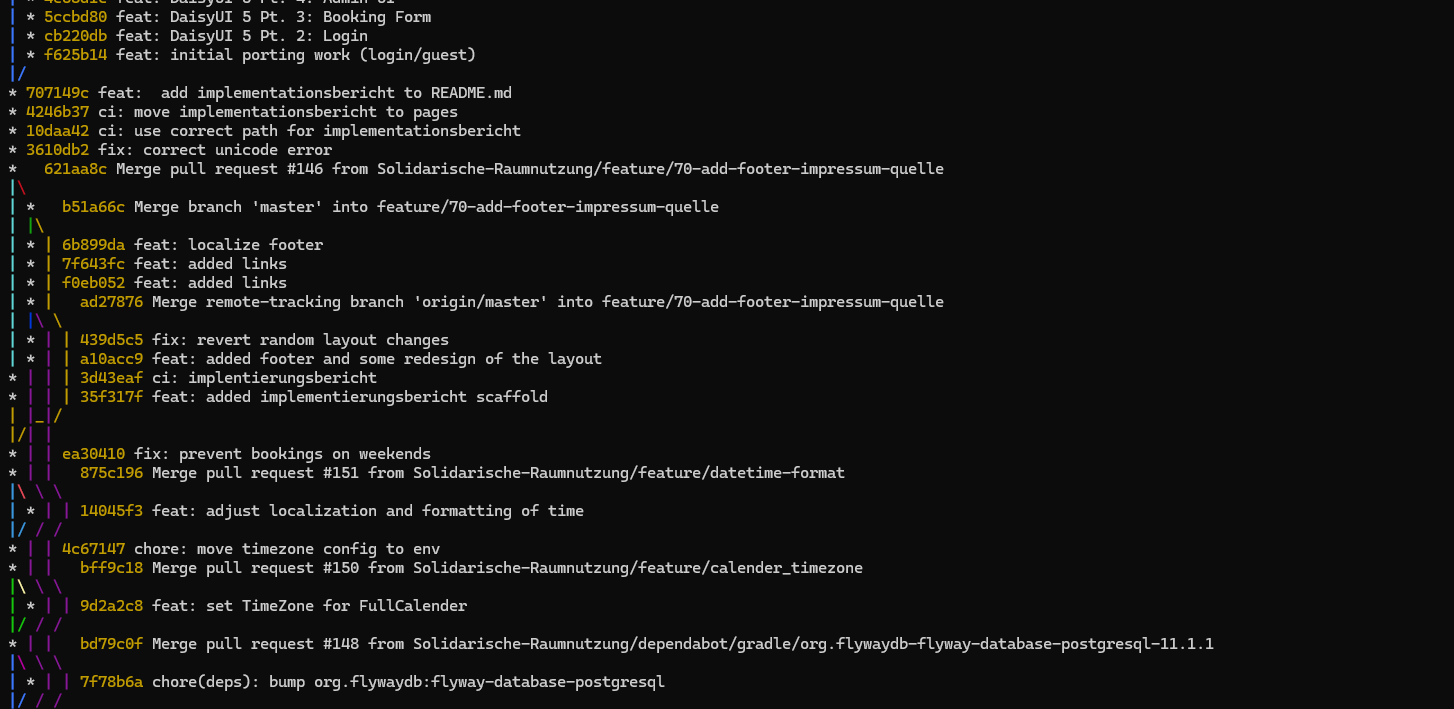
\includegraphics[width=1\linewidth]{image.png}
            \label{fig:enter-label}
        \end{figure}
    \end{frame}
    
    
    \section{Fragen?}
    
    \end{document}
